\documentclass[landscape,paperwidth=48in,paperheight=36in,fontscale=0.3]{baposter}

\usepackage{times}
\usepackage{calc}
\usepackage{url}
\usepackage{graphicx}
\usepackage{amsthm}
\usepackage{amsmath}
\usepackage{amssymb}
\usepackage{relsize}
\usepackage{multirow}
\usepackage{multicol}
\usepackage{booktabs}
\usepackage{microtype}
\usepackage{graphicx}

\usepackage[T1]{fontenc}
\usepackage{ae}
\usepackage{enumitem}
\usepackage{colortbl}
\usepackage{xcolor}
\usepackage{tcolorbox}
\usepackage[vlined]{algorithm2e}
\usepackage{minted}
\let\vec\mathbf
\setlength{\algomargin}{0pt}

\setlist[itemize]{leftmargin=*,nosep}
\setlength{\columnsep}{0.7em}
\setlength{\columnseprule}{0mm}

\setlist[enumerate]{leftmargin=2.3em,nosep}
\setlength{\columnsep}{0.5em}
\setlength{\columnseprule}{0mm}

% \setlength{\paperwidth}{60in} % A0 width: 46.8in
% \setlength{\paperheight}{36in} % A0 height: 33.1in

% \renewcommand{\rmdefault}{ptm} % Arial
% \renewcommand{\sfdefault}{ptm} % Arial
\renewcommand{\familydefault}{\sfdefault}

% define colors
\usepackage{colortbl}
\usepackage{xcolor}
\newcommand{\highlight}[2][yellow]{\mathchoice%
  {\colorbox{#1}{$\displaystyle#2$}}%
  {\colorbox{#1}{$\textstyle#2$}}%
  {\colorbox{#1}{$\scriptstyle#2$}}%
  {\colorbox{#1}{$\scriptscriptstyle#2$}}}%
  
\definecolor{ctitle}{HTML}{000000}
\definecolor{mypurple}{RGB}{223, 204, 251}
\definecolor{imptext}{RGB}{103, 65, 136} %116, 9, 56
\definecolor{rowcolor}{RGB}{209, 233, 246}
\definecolor{subtitlecolor}{RGB}{11, 47, 159}
\definecolor{mathcolor}{RGB}{209, 233, 246}
\definecolor{mathcolor2}{RGB}{238, 202, 213}
\begin{document}

\begin{poster}{
 % Show grid to help with alignment
 grid=false,
 columns=4,
 % Column spacing
 colspacing=0.7em,
 % Color style
 headerColorOne=mypurple,
 borderColor=mypurple,
 % Format of textbox
 textborder=faded,
 % Format of text header
 headerborder=open,
 headershape=roundedright,
 headershade=plain,
 background=none,
 bgColorOne=cyan!10!white,
 headerheight=0.15\textheight}
 {
    \makebox[0.01\textwidth]{}
    \includegraphics[width=0.08\linewidth]{logo/huawei.png}
    
\includegraphics[width=0.075\linewidth]{logo/vdsr_enhanced.jpg}
 }
% Title
{
    \\[0.3em]\sc\huge\bf Learning Truncated Causal History Model for Video Restoration
}
% Authors
{
\vspace{0.3em} Amirhosein Ghasemabadi$^{\clubsuit1,2}$ \enspace Muhammad Kamran Janjua$^{\clubsuit2}$ \enspace Mohammad Salameh$^2$ \enspace Di Niu$^1$ \\[0.2em]
{$^1$ECE Department, University of Alberta \enspace$^2$Huawei Technologies, Canada \\[0.1em] \(\clubsuit\) indicates equal contribution}
}
% University logo
{
    \begin{tabular}{c}
        \raisebox{-0.9\height}{
\includegraphics[width=0.14\linewidth]{logo/nips}}\\[0.5em]
        \raisebox{-0.5\height}{
\includegraphics[width=0.12\linewidth]{logo/link.pdf}\hspace{0.002\linewidth}
\includegraphics[height=0.05\linewidth]{logo/turtle_qr_code.png}}
    \end{tabular}
}
\headerbox{\bf\color{ctitle}Overview}{name=summary,column=0,row=0,span=1}{
    \begin{minipage}[c]{\textwidth}
        \begin{itemize}

            \item \textbf{Video Restoration Challenges}: \begin{itemize} 
                \item Effective information fusion across frames. 
                \item Handling the complexity of non-uniform motion between frames. 
            \end{itemize}

            \item \textbf{Traditional methods} process a range of contextual frames either in \textbf{parallel}, leading to increased memory and inference costs or with \textbf{recurrence}, which results in error accumulation and limited parallelism.

            \item To handle motion, methods in literature employ optical flow to explicitly estimate motion, however, optical flow suffers on degraded videos.

            % \item \textbf{\textsc{TURTLE}} introduces the Causal History Model (CHM), which efficiently aligns and borrows information from previously processed frames by summarizing a truncated history of the earlier frames into an evolving state. 

            \item \textbf{\textsc{TURTLE}} introduces the Causal History Model (CHM), which efficiently \textcolor{imptext}{borrows information} from a truncated history of previously processed frames by implicitly compensating motion, maintaining high restoration quality while \textcolor{imptext}{significantly reducing memory and computational costs}.

            \item \textbf{\textsc{TURTLE}}  achieves state-of-the-art results on multiple video restoration benchmarks.
        \end{itemize} 
    \end{minipage}
}

%%%%%%%%%%%%%%%%%%%%%%%%%%%%%%%%%%%%%%%%%%%%%%%%%%%%%%%%%%%%%%%%%%%%%%%%%%%
\headerbox{\bf\color{ctitle}Method}{name=method,column=1,row=0,span=1}{
% \textbf{\color{blue}AMP: Adversarial Model Perturbation}\\
\begin{itemize}
    \item \textsc{TURTLE} adopts a causal design to process frames online. \textsc{TURTLE}'s encoder is historyless i.e., it only processes a single frame, while the decoder stacks \textsf{CHM} blocks as blackboxes at several stages. 
    \item The decoder, therefore, conditions the restoration on the history of the input frame due to \textsf{CHM}.
\end{itemize}
\begin{minipage}{0.99\linewidth}
\centering
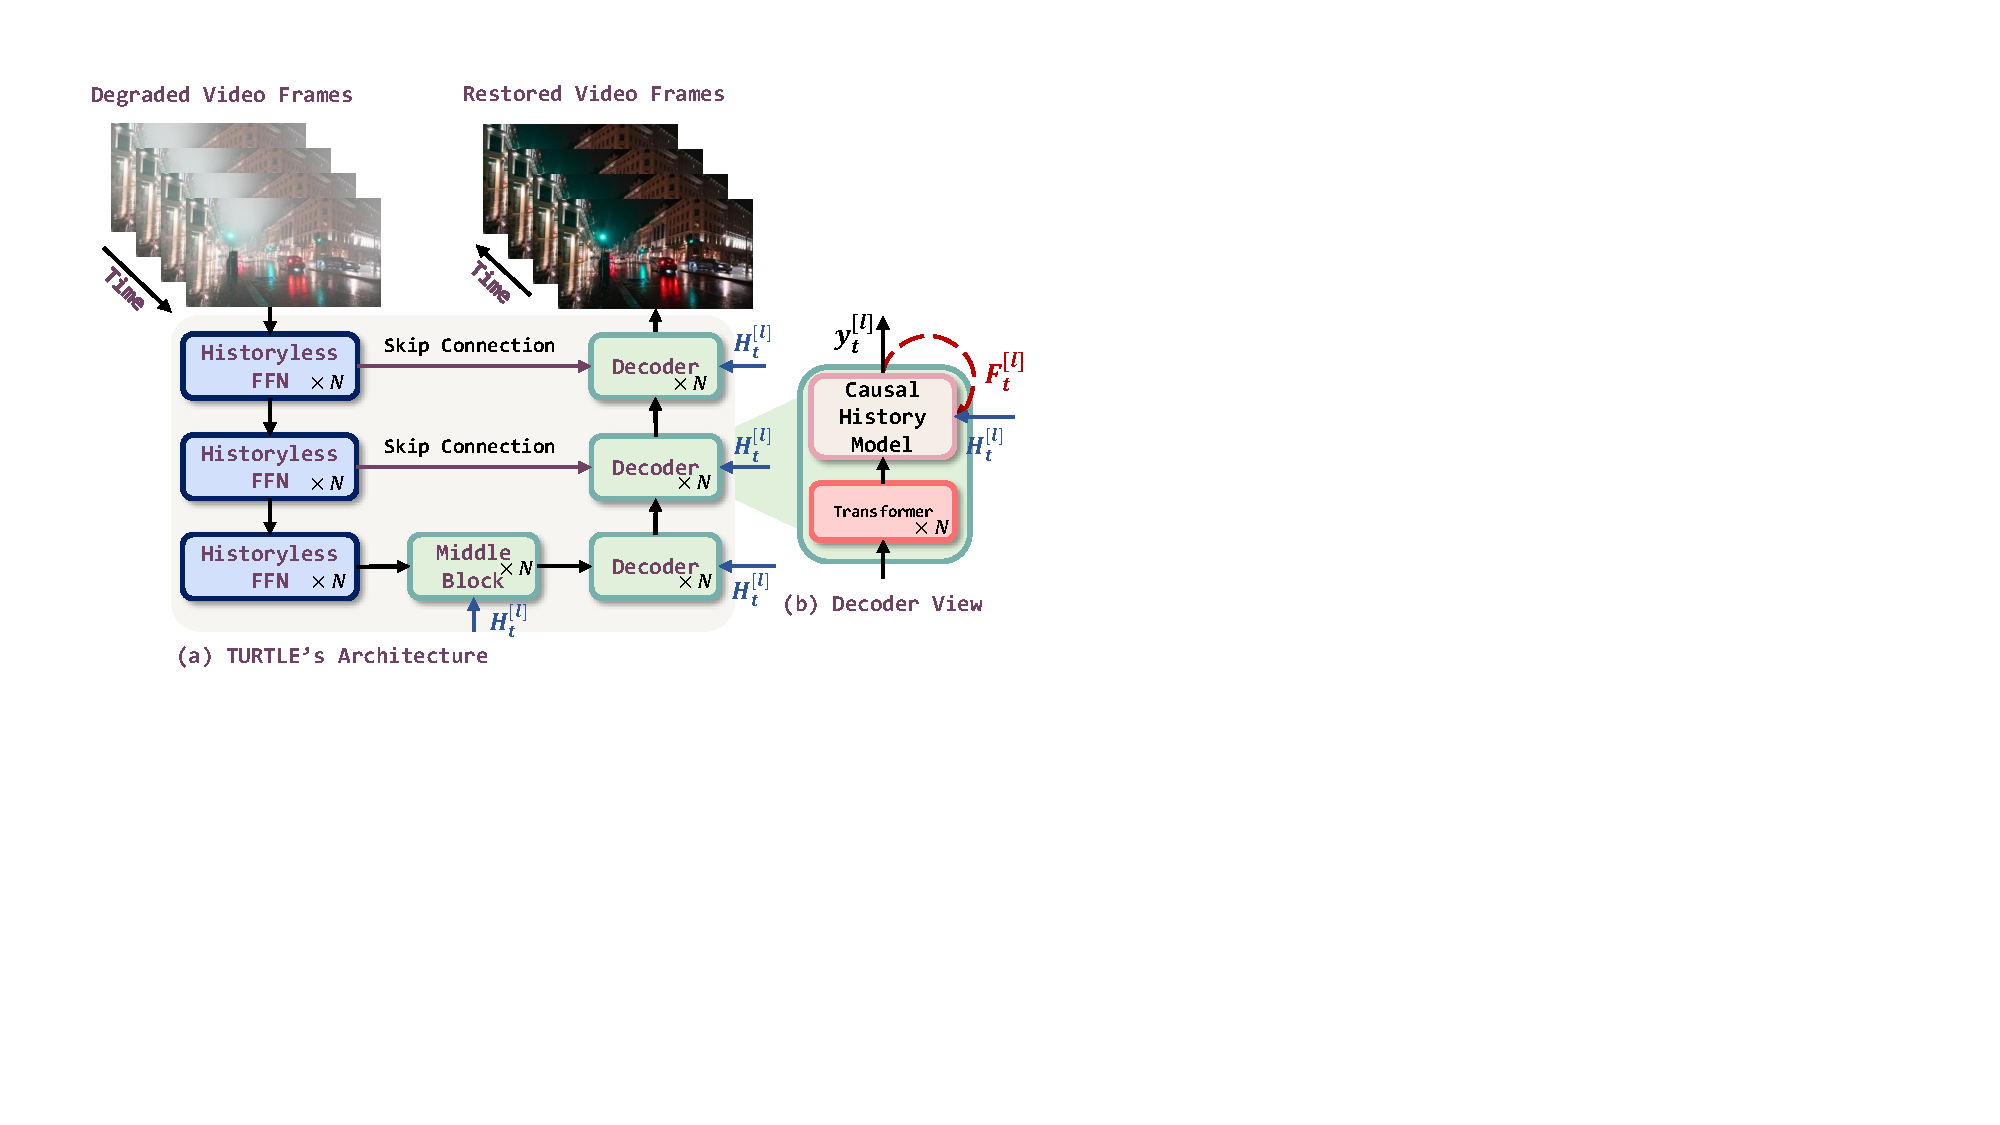
\includegraphics[width=\linewidth]{new_imgs/arch.pdf}
\end{minipage}
}

%%%%%%%%%%%%%%%%%%%%%%%%%%%%%%%%%%%%%%%%%%%%%%%%%%%%%%%%%%%%%%%%%%%%%%%%%%%
\headerbox{\bf\color{ctitle}Experiments}{name=results,column=2,row=0,span=2}{
\begin{minipage}{0.9\linewidth}
\textbf{\color{blue}Results on Video Restoration Tasks:}
\vspace{0.5em}
\end{minipage}

\begin{minipage}{0.33\linewidth}
\centering
\resizebox{.95\linewidth}{!}{%
\begin{tabular}{lcc}
\toprule
\textbf{Methods} & \textbf{PSNR} (\(\uparrow\)) & \textbf{SSIM} (\(\uparrow\))  \\
\midrule
HRIR & 16.83 & 0.6402 \\
WeatherDiff & 20.98 & 0.6697 \\
FDM & 23.49 & 0.7657 \\
MetaRain (Scrt) & 22.21 & 0.6723 \\
MetaRain (Meta) & 23.49 & 0.7171 \\
NightRain & \underline{26.73} & \underline{0.8647} \\
\rowcolor{rowcolor} \textbf{\textsc{TURTLE}} & \textbf{29.26} & \textbf{0.9250} \\
\midrule
\textbf{Methods} & \textbf{PSNR} (\(\uparrow\)) & \textbf{SSIM} (\(\uparrow\))  \\
\midrule
EDVR & 17.93 & 0.5790 \\
BasicVSR & 22.46 & 0.8473 \\
RDDNet & 22.97 & 0.8742 \\
BasicVSR\(++\) & 22.64 & 0.8618 \\
RVRT & 20.90 & 0.7974 \\
SVDNet & \underline{25.06} & \underline{0.9210} \\
\rowcolor{rowcolor} \textbf{\textsc{TURTLE}} & \textbf{26.02} & \textbf{0.9230} \\
\bottomrule
\end{tabular}
}

\vspace{0.5em}
(a) Night Deraining \& Desnowing
\vspace{0.5em}
\end{minipage}
\begin{minipage}{0.33\linewidth}
\centering
\resizebox{.87\linewidth}{!}{%
\begin{tabular}{lcc}
\toprule
\textbf{Methods} & \textbf{PSNR} (\(\uparrow\)) & \textbf{SSIM} (\(\uparrow\))  \\
\midrule
STRCNN & 29.42 & 0.8930 \\
DBN & 31.21 & 0.9220 \\
IFI-RNN & 30.89 & 0.8820 \\
CDVD-TSP & \underline{31.58} & \underline{0.9260} \\
PVDNet & 31.35 & 0.9230 \\
ESTRNN & 31.39 & \underline{0.9260} \\
\rowcolor{rowcolor} \textbf{\textsc{TURTLE}} & \textbf{33.58} & \textbf{0.9540} \\
\midrule
\textbf{Methods} & \textbf{PSNR} (\(\uparrow\)) & \textbf{SSIM} (\(\uparrow\))  \\
\midrule
ESTRNN & 31.07 & 0.9023 \\
EDVR & 31.54 & 0.9260 \\
FGST & 32.90 & 0.9610 \\
BasicVSR\(++\) & 34.01 & 0.9520 \\
GSTA & 32.10 & 0.9600 \\
DSTNet & \underline{34.16} & \underline{0.9679} \\
\rowcolor{rowcolor} \textbf{\textsc{TURTLE}} & \textbf{34.50} & \textbf{0.9720} \\
\bottomrule
\end{tabular}
}

\vspace{0.5em}
(b) Real \& Synthetic Deblurring
\vspace{0.5em}
\end{minipage}
\begin{minipage}{0.33\linewidth}
\centering
\resizebox{.87\linewidth}{!}{%
\begin{tabular}{lcc}
\toprule
\textbf{Methods} & \textbf{PSNR} (\(\uparrow\)) & \textbf{SSIM} (\(\uparrow\))  \\
\midrule
VRT & 27.77 & 0.8856 \\
TTVSR & 28.05 & 0.8998 \\
RVRT & 28.24 & 0.8857 \\
BasicVSR\(++\) & 29.75 & 0.9171 \\
RDDNet & 28.38 & 0.9096 \\
ViMPNet & \underline{31.02} & \underline{0.9283} \\
\rowcolor{rowcolor} \textbf{\textsc{TURTLE}} & \textbf{32.01} & \textbf{0.9590} \\
\midrule
\textbf{Methods} & \textbf{PSNR} (\(\uparrow\)) & \textbf{SSIM} (\(\uparrow\))  \\
\midrule
EDVR & 23.51 & 0.7492 \\
MANA & 23.15 & 0.7513 \\
TTVSR & 23.60 & 0.7686 \\
BasicVSR\(++\) & 23.70 & 0.7713 \\
EAVSR & 23.61 & 0.7618 \\
EAVSR\(+\) & \underline{23.94} & \underline{0.7726} \\
\rowcolor{rowcolor} \textbf{\textsc{TURTLE}} & \textbf{25.30} & \textbf{0.8272} \\
\bottomrule
\end{tabular}
}

\vspace{0.5em}
(c) Raindrop Removal \& SR 
\vspace{0.5em}
\end{minipage}

\begin{minipage}{0.34\linewidth}
\textbf{\color{blue}Ablation Studies:}
\vspace{0.5em}
\end{minipage}
\begin{minipage}{0.65\linewidth}
\textbf{{\color{blue}Profiling \textsc{TURTLE}:}}
\vspace{0.5em}
\end{minipage}

\begin{minipage}{0.34\linewidth}
\centering
\resizebox{.9\linewidth}{!}{%
\begin{tabular}{@{}lll@{}}
\toprule
\textbf{Ablation Studies} & \textbf{Configurations} & \textbf{PSNR} (\(\uparrow\)) \\ \midrule
\multirow{3}{*}{State Align Block} & No \textsf{CHM} & 31.84 \\
 & No \(\phi\) & 32.07 \\
 & \textsc{TURTLE} & 32.36 \\ \midrule
\multirow{3}{*}{\begin{tabular}[c]{@{}l@{}}Truncation\\ Factor \(\tau\)\end{tabular}} & 1 & 32.15 \\
 & 5 & 32.26 \\
 & 3 (\textsc{TURTLE}) & 32.26 \\ \midrule
\multirow{3}{*}{k in \textit{topk}} & 1 & 32.18 \\
 & 20 & 32.10 \\
 & 5 (\textsc{TURTLE}) & 32.26 \\ \bottomrule
\end{tabular}
}
\end{minipage}
\begin{minipage}{0.65\linewidth}
\centering
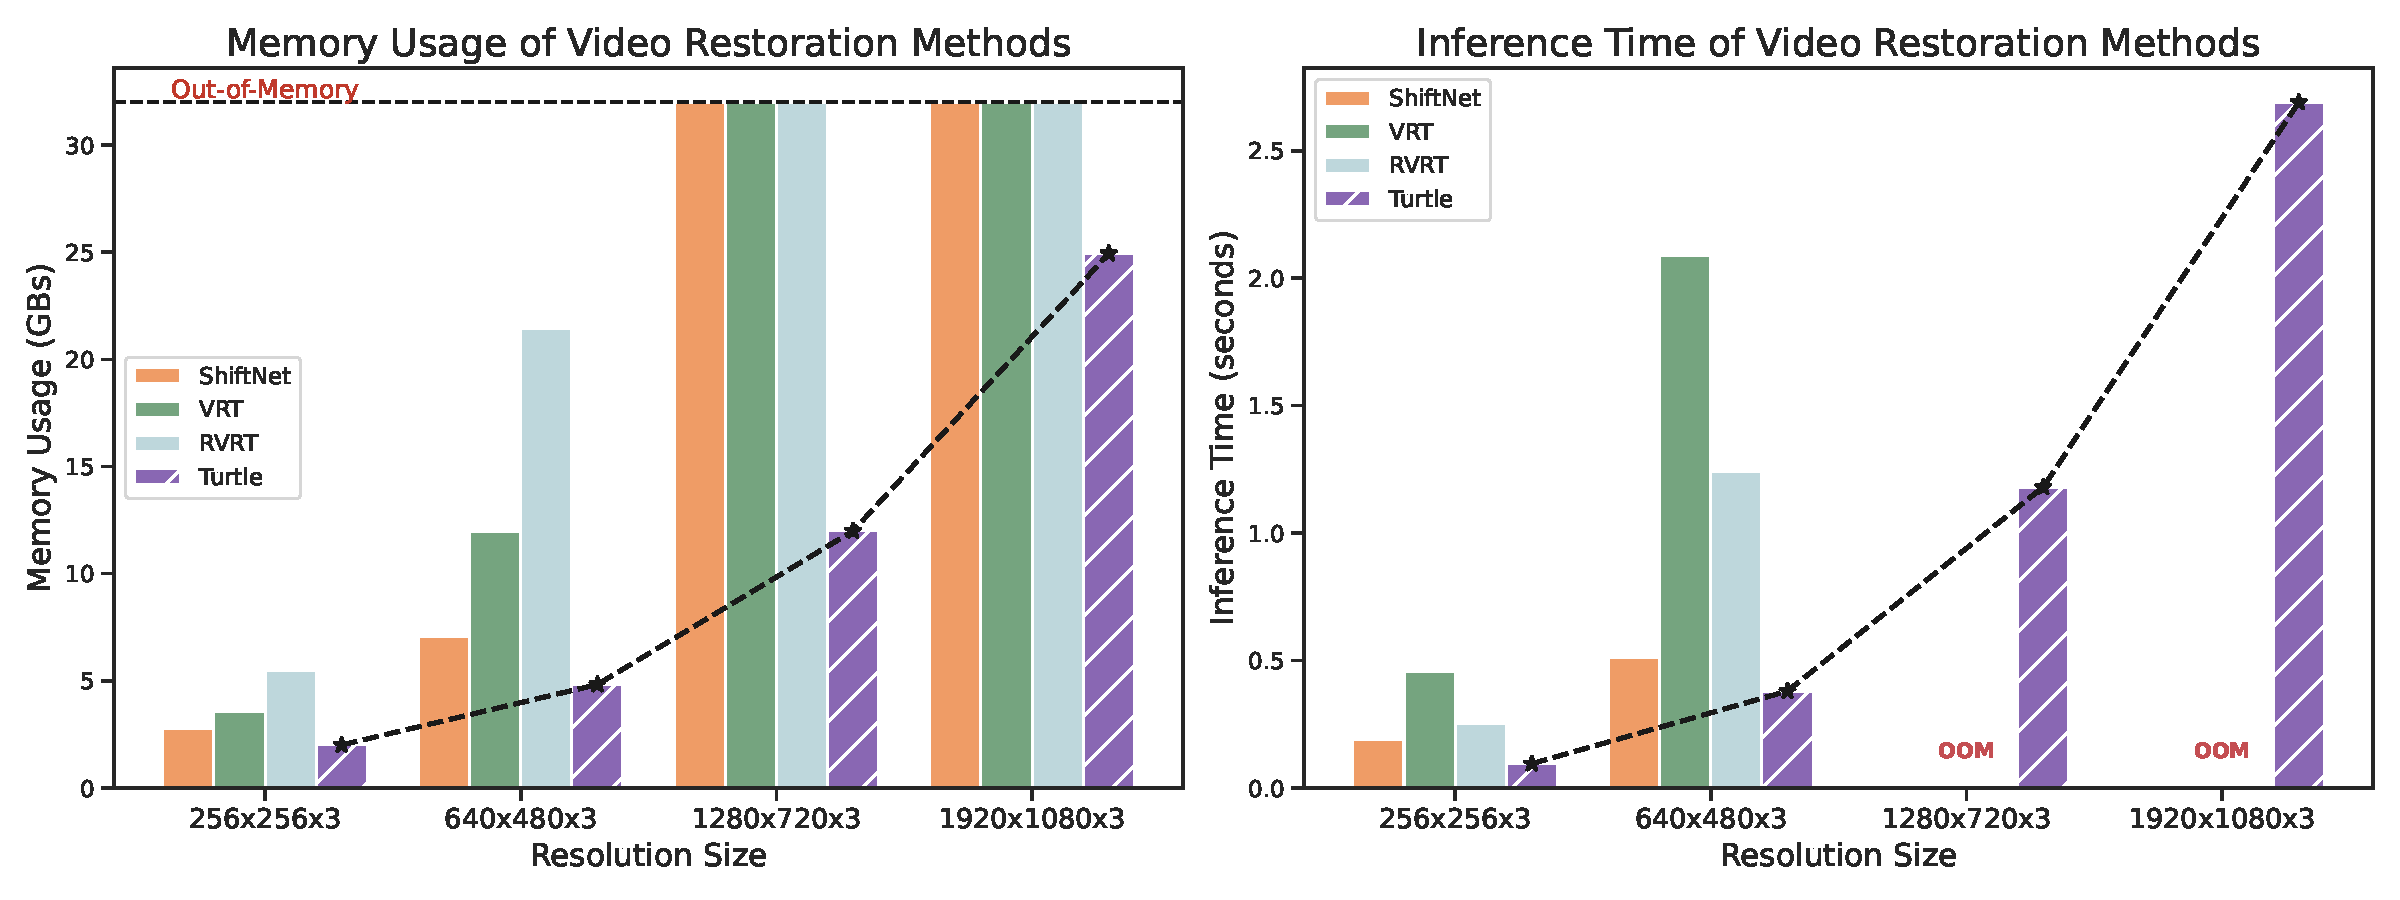
\includegraphics[width=\linewidth]{new_imgs/memory_inf_comp1.pdf}
\end{minipage}

\begin{minipage}[t]{.7\linewidth}
\begin{minipage}{\linewidth}
\vspace{0.5em}
\textbf{\color{blue}Video Deblurring, Raindrop, \& Desnowing Results:}
\vspace{0.5em}
\end{minipage}
\begin{minipage}{0.99\linewidth}
    \begin{minipage}{\linewidth}
    \centering
    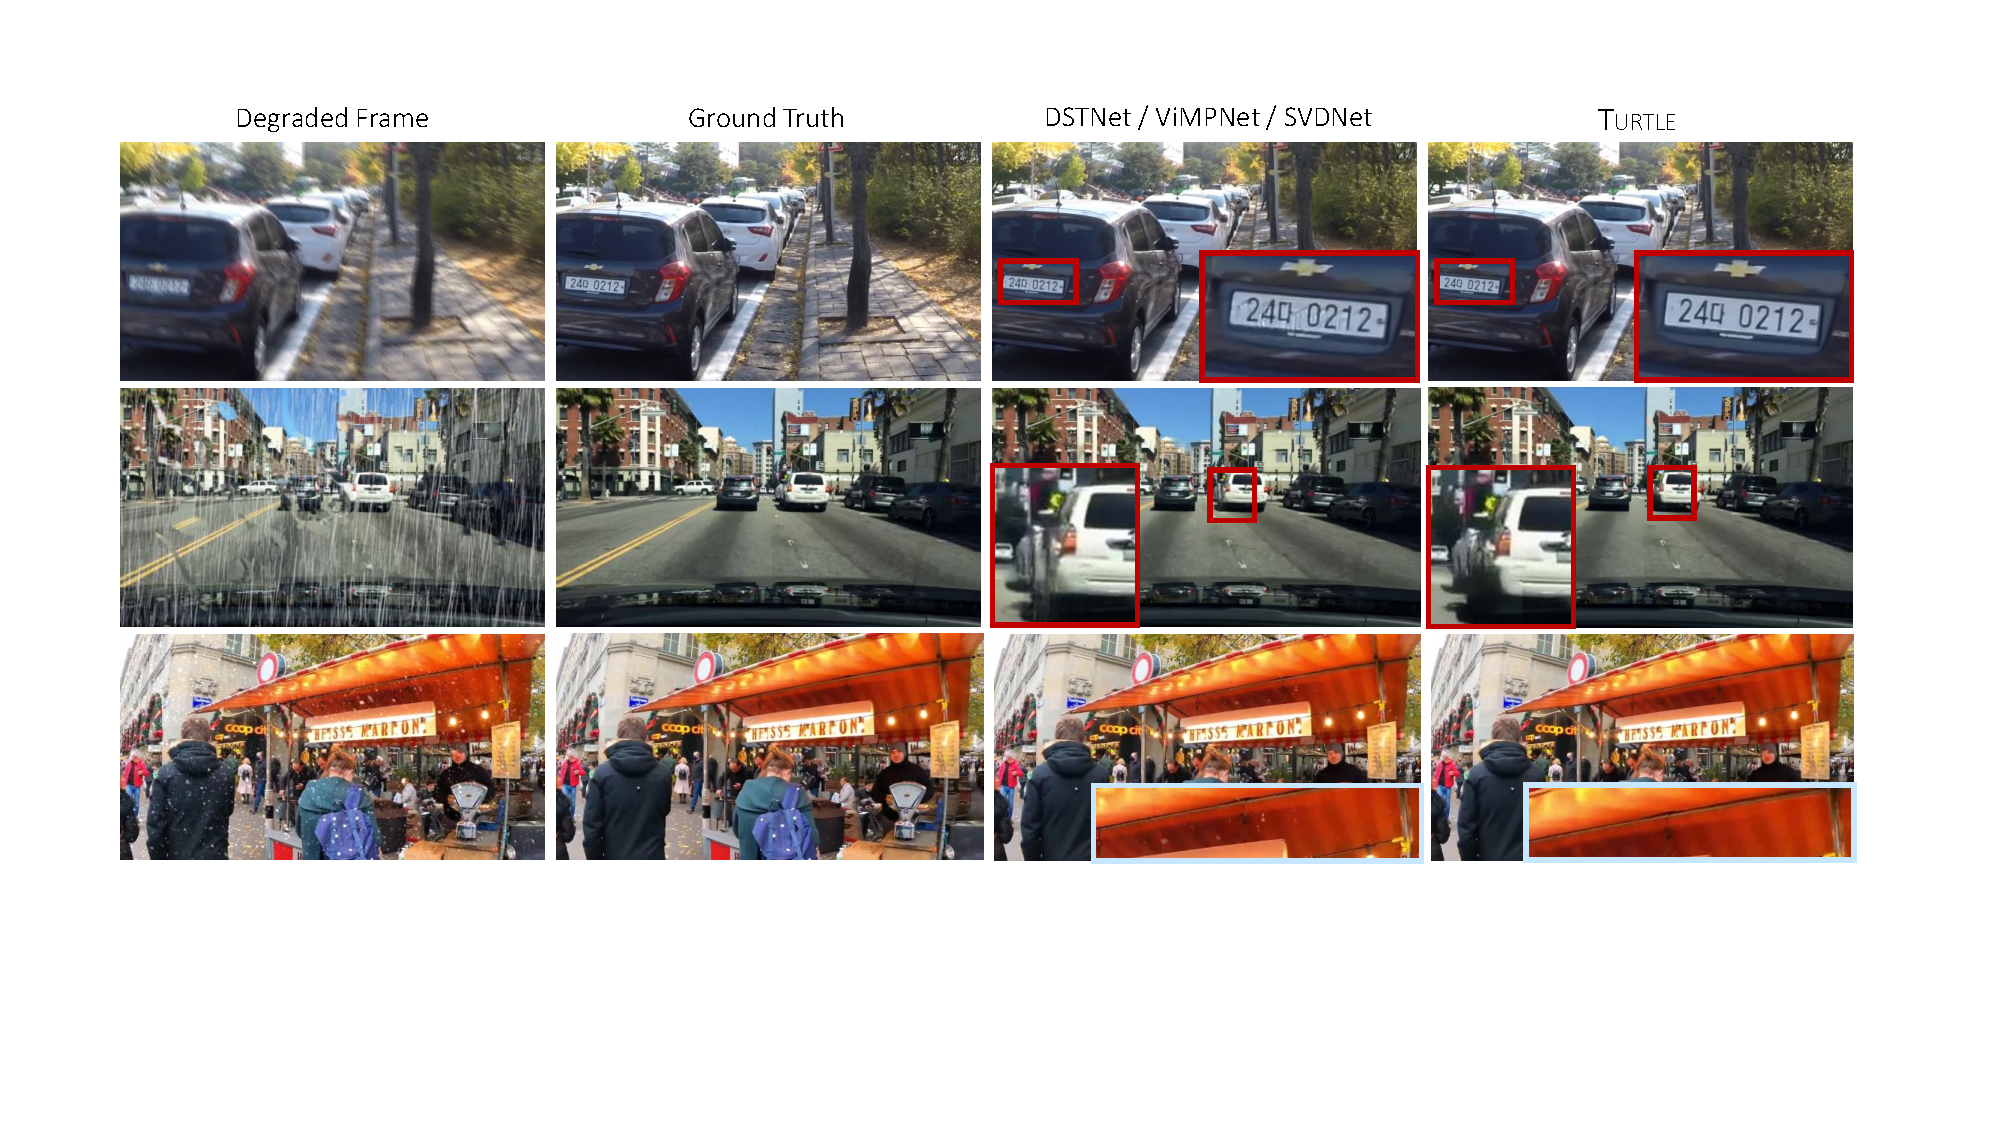
\includegraphics[width=.99\linewidth]{new_imgs/main_fig_01.pdf}
    \end{minipage}
\end{minipage}
\\
\begin{minipage}{\linewidth}
\vspace{0.5em}
\textbf{\color{blue}Real-World Restoration Results:}
\vspace{0.5em}
\end{minipage}
\begin{minipage}{0.99\linewidth}
    \begin{minipage}{\linewidth}
    \centering
    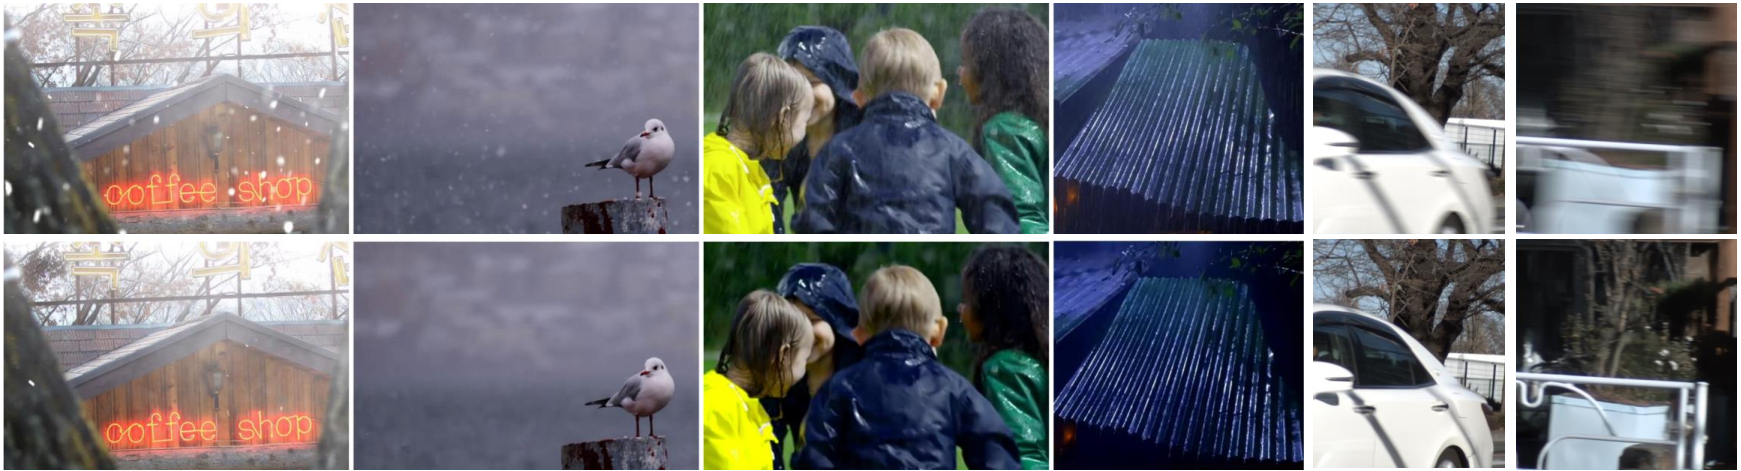
\includegraphics[width=.99\linewidth]{new_imgs/main_fig_02.pdf}
    \end{minipage}
\end{minipage}
\end{minipage}
\begin{minipage}[t]{.24\linewidth}
\small
\textbf{\color{blue}Denoising Results:}\\
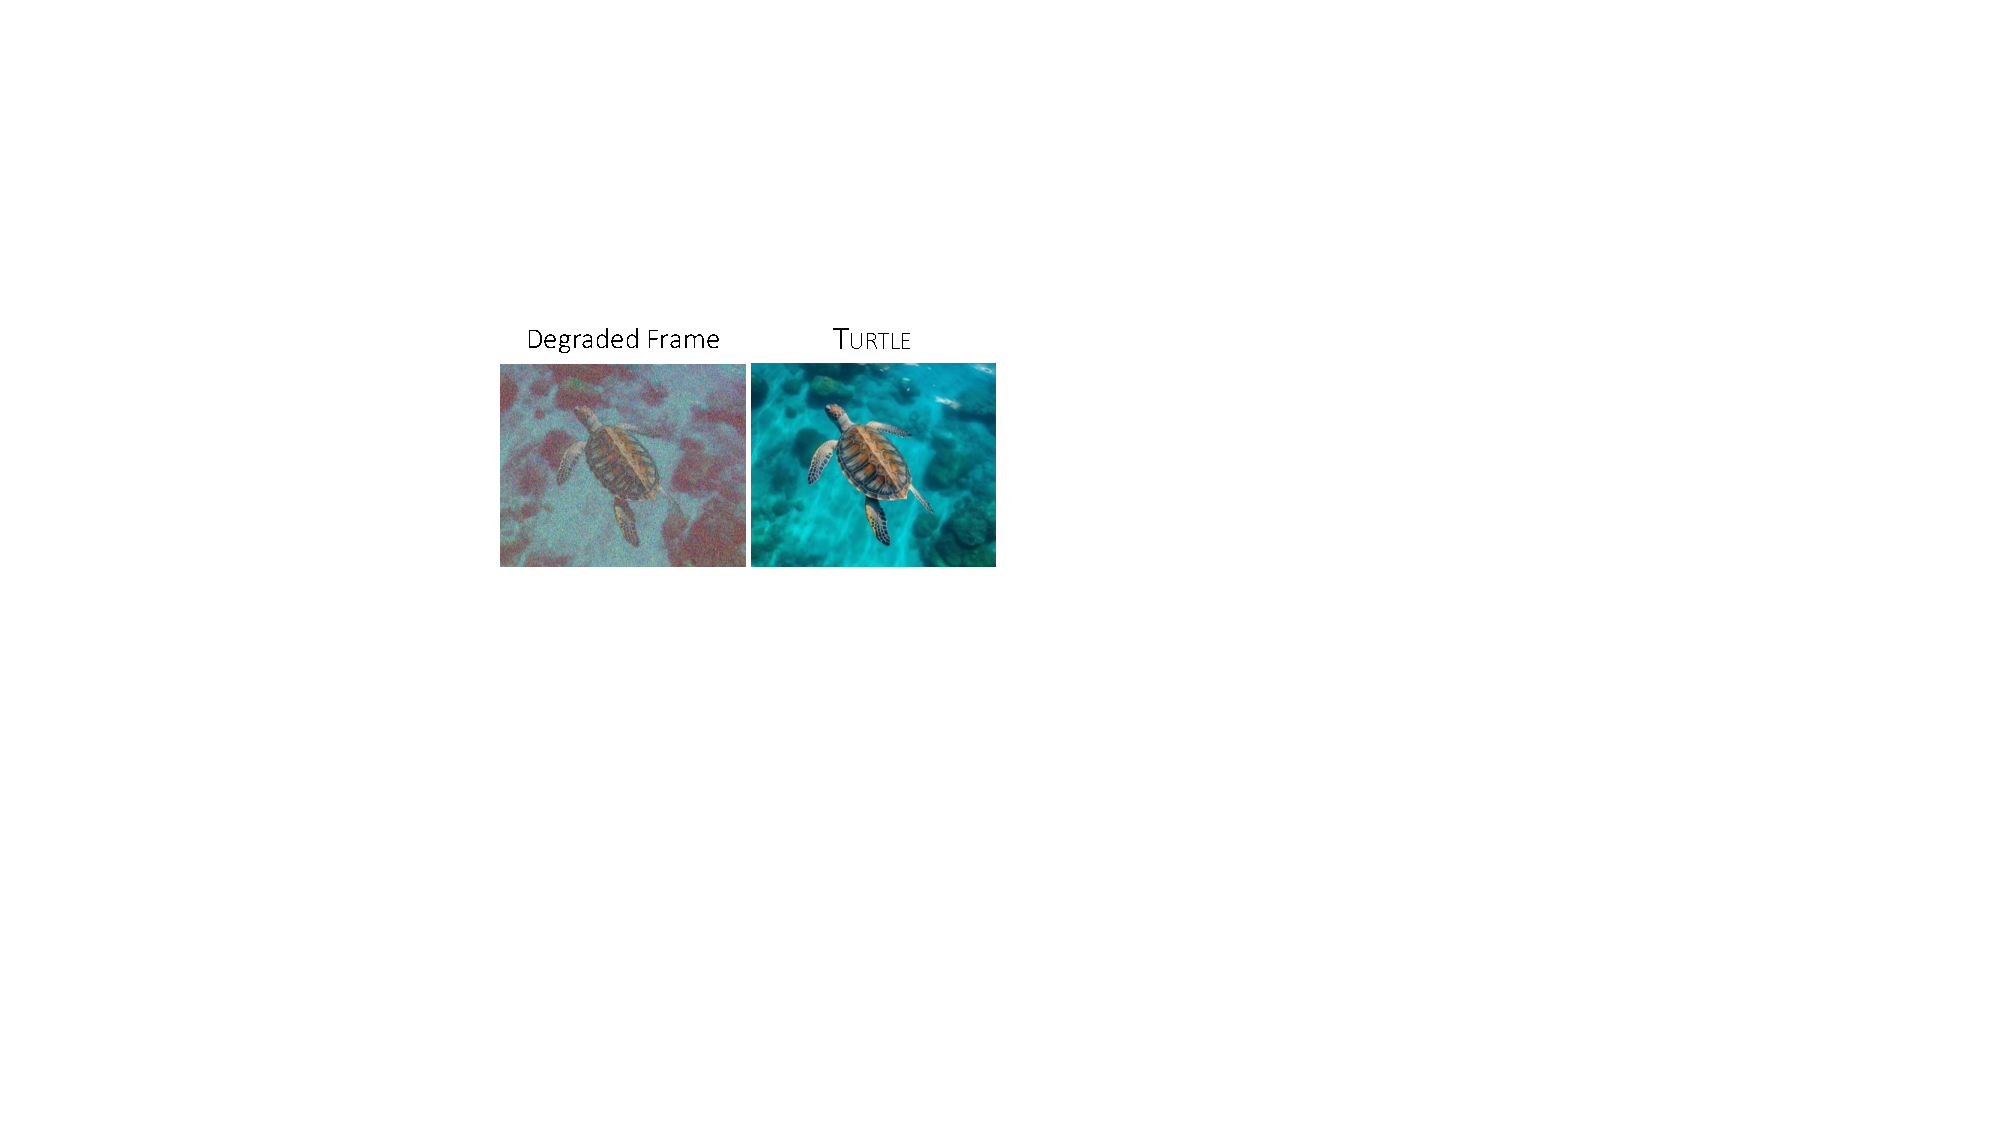
\includegraphics[width=1.2\linewidth]{new_imgs/turtle_denoise.pdf}
\vspace{2em}
\textbf{\color{blue}References:}\\
\vspace{-2em}
\begin{enumerate}[label={[\arabic*]}]
    \item Liang \textit{et al}. Recurrent video restoration transformer with guided deformable attention. NeurIPS 22.
    \item Li \textit{et al}. A simple baseline for video restoration with grouped spatial-temporal shift. CVPR 23.
    \item Liang \textit{et al}. Vrt: A video restoration transformer. TIP 24.
\end{enumerate}
\end{minipage}
}

%%%%%%%%%%%%%%%%%%%%%%%%%%%%%%%%%%%%%%%%%%%%%%%%%%%%%%%%%%%%%%%%%%%%%%%%%%%
\headerbox{\bf\color{ctitle}Causal History Model (\textsf{CHM})}{name=algorithm,column=0,row=0.4,span=1}{
        \begin{itemize}
            \item Causal History Model \textcolor{imptext}{extends the state-space modeling paradigm to video processing.} CHM processes videos online and in streaming fashion.
            \item \textbf{\textsf{CHM} models the evolving state and compensates the history for motion} relative to the input and learns to re-weight information in the history.
            \item The \textbf{causal design in \textsc{Turtle} enables recurrence in inference} through state-memorized historical features (stateful configuration); \textbf{while allowing parallel training} by sampling short video clips (stateless configuration).
            \item \textbf{\textsc{TURTLE}'s encoder processes each frame individually}, while its decoder reuses features from previously restored frames, based on the proposed Causal History Model (CHM).
        \end{itemize}
        \begin{align}
            \label{eq:chm}
            \vec{\hat{H}}_{t}^{[l]} &= \highlight[mathcolor]{\phi_{t}(\vec{H}_{t}^{[l]}, \vec{F}_{t}^{[l]})} \oplus \mathcal{B}_{t}(\vec{F}_{t}^{[l]}), \\
            \label{eq:chm2}
            \vec{y}_t^{[l]} &= \highlight[mathcolor2]{\psi_{t}(\vec{\hat{H}}_{t}^{[l]}, \vec{F}_{t}^{[l]})} + \mathcal{D}_{t}(\vec{F}_{t}^{[l]}).
        \end{align}
        \begin{itemize}
            \item \textbf{\(\highlight[mathcolor]{\text{State Align Block}~\phi}\)}: implicitly tracks and aligns the \textit{topk} most relevant regions in the history with the input frame. Therefore, \(\phi\) compensates for motion the input with respect to the trajectory and establishes \textit{one-to-topk} correspondence.
            \item \textbf{\(\highlight[mathcolor2]{\text{Frame History Router }~\psi}\)}: re-weights the motion compensated history along with the input, thereby encouraging \& accentuating relevant information.
        \end{itemize}
}
%%%%%%%%%%%%%%%%%%%%%%%%%%%%%%%%%%%%%%%%%%%%%%%%%%%%%%%%%%%%%%%%%%%%%%%%%%%%%
\headerbox{\bf\color{ctitle}Is \textsc{CHM} Necessary?}{name=method,column=1,row=0.4,span=1,boxpadding=0.45em}{
\textbf{\color{blue}\textsf{CHM} Procedure:}
% \textsf{CHM} utilizes attention mechanism to compute region-wise correspondences in the history, and to re-weight the entire trajectory. However, in the first case, CHM limits the lookback window to \textit{topk} most similar regions to avoid spurious correlations hampering the flow of useful information.
\begin{itemize}
    \item \textsf{CHM} utilizes an attention mechanism to compute region-wise correspondences in the history and to re-weight the entire trajectory.
    \item However, \textsf{CHM} limits the lookback window to the \textit{top-k} most similar regions to avoid spurious correlations that may hamper the flow of useful information.
\end{itemize}

\begin{minipage}{\linewidth}
    \centering
    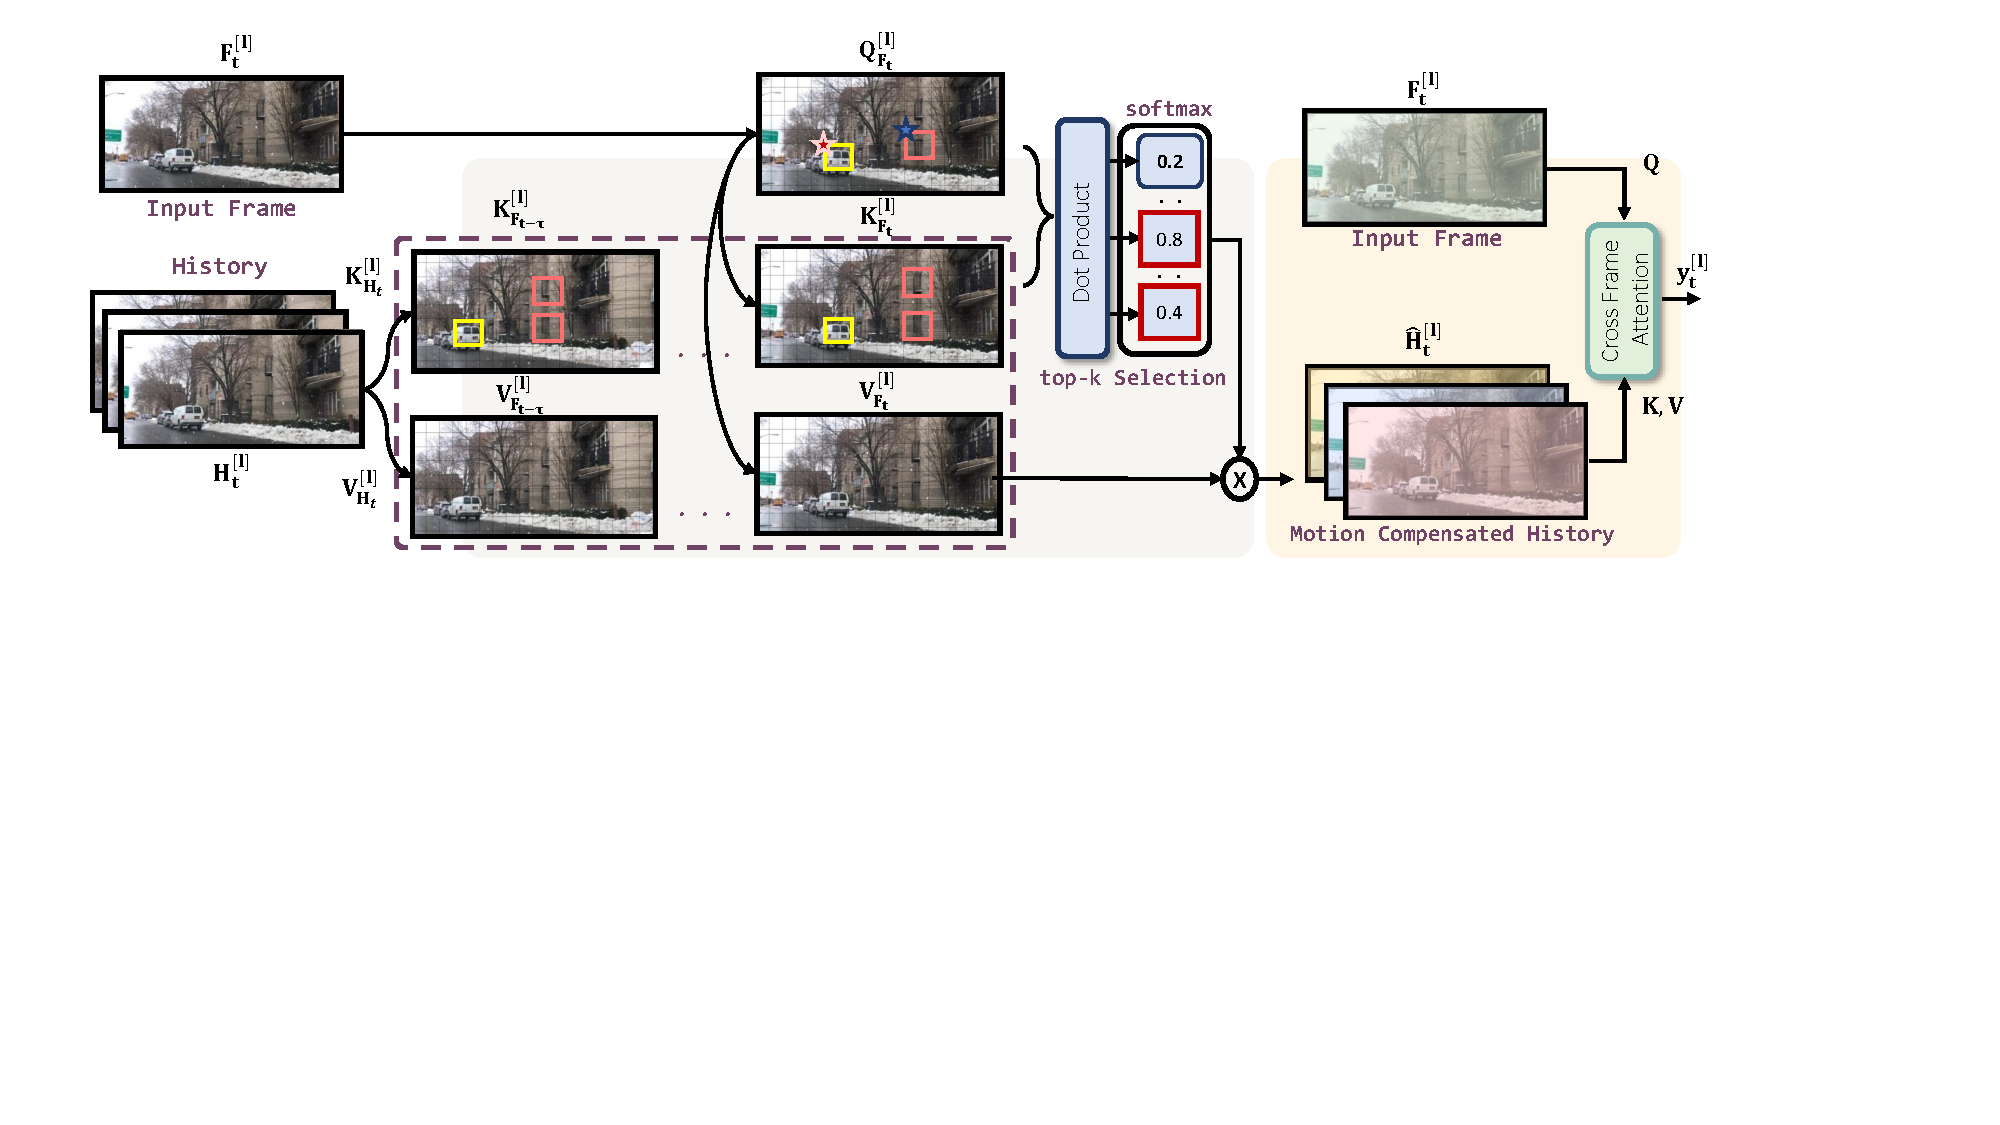
\includegraphics[width=.99\linewidth]{new_imgs/chm.pdf}
\end{minipage}
\vspace{0.4em}
\textbf{\color{blue}\textsf{CHM}'s Motivation:} 
\begin{itemize}
    \item We ablate the necessity of \textsf{CHM} for achieving high perceptual quality in restoration results.
    \item In cases where specific regions in the current frame (input) are occluded, \textsf{CHM} retrieves similar information from past frames to restore the occluded areas.
\end{itemize}
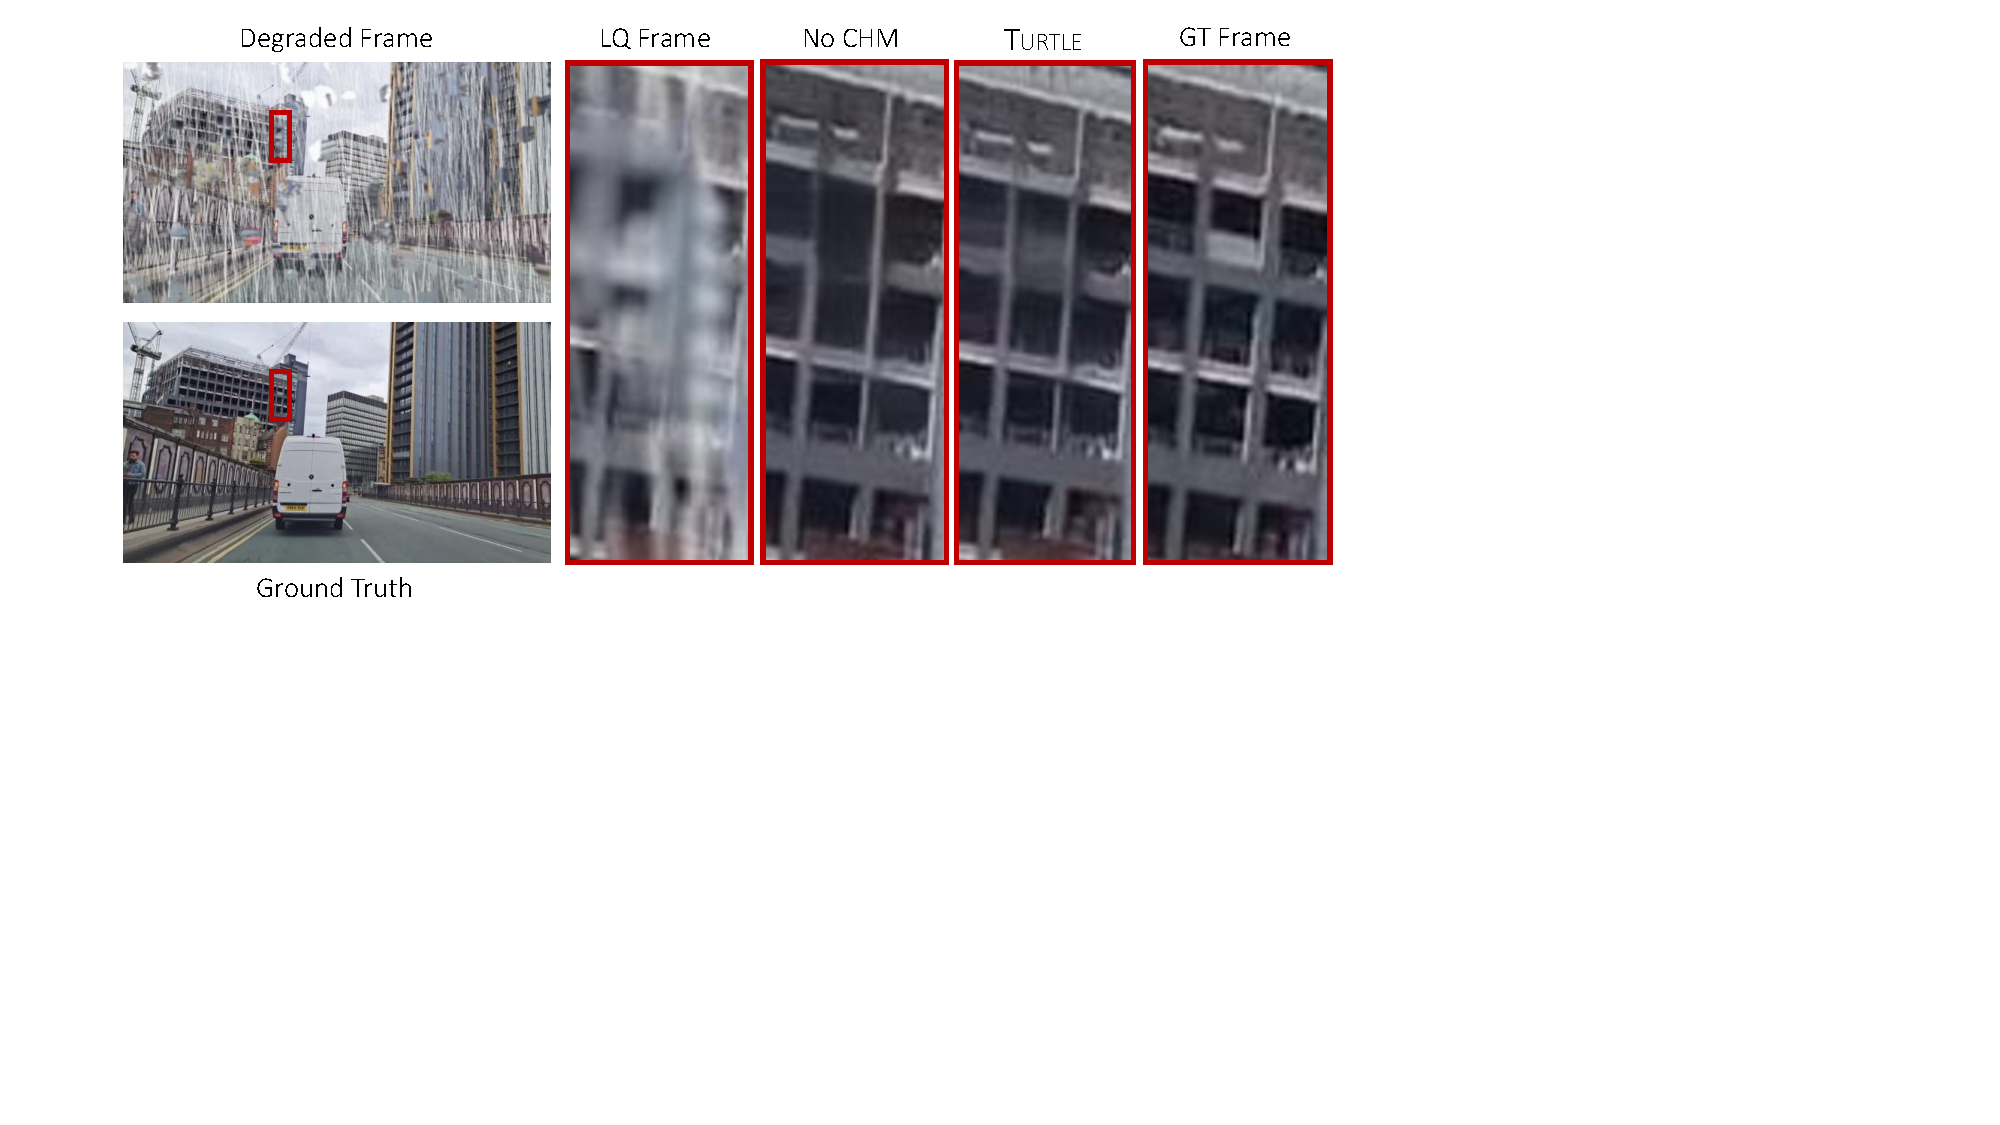
\includegraphics[width=.99\linewidth]{new_imgs/nochm_diag.pdf}

}
\end{poster}
\end{document}